\documentclass[tikz,border=10pt]{standalone}
\usetikzlibrary{arrows.meta,positioning}

\begin{document}
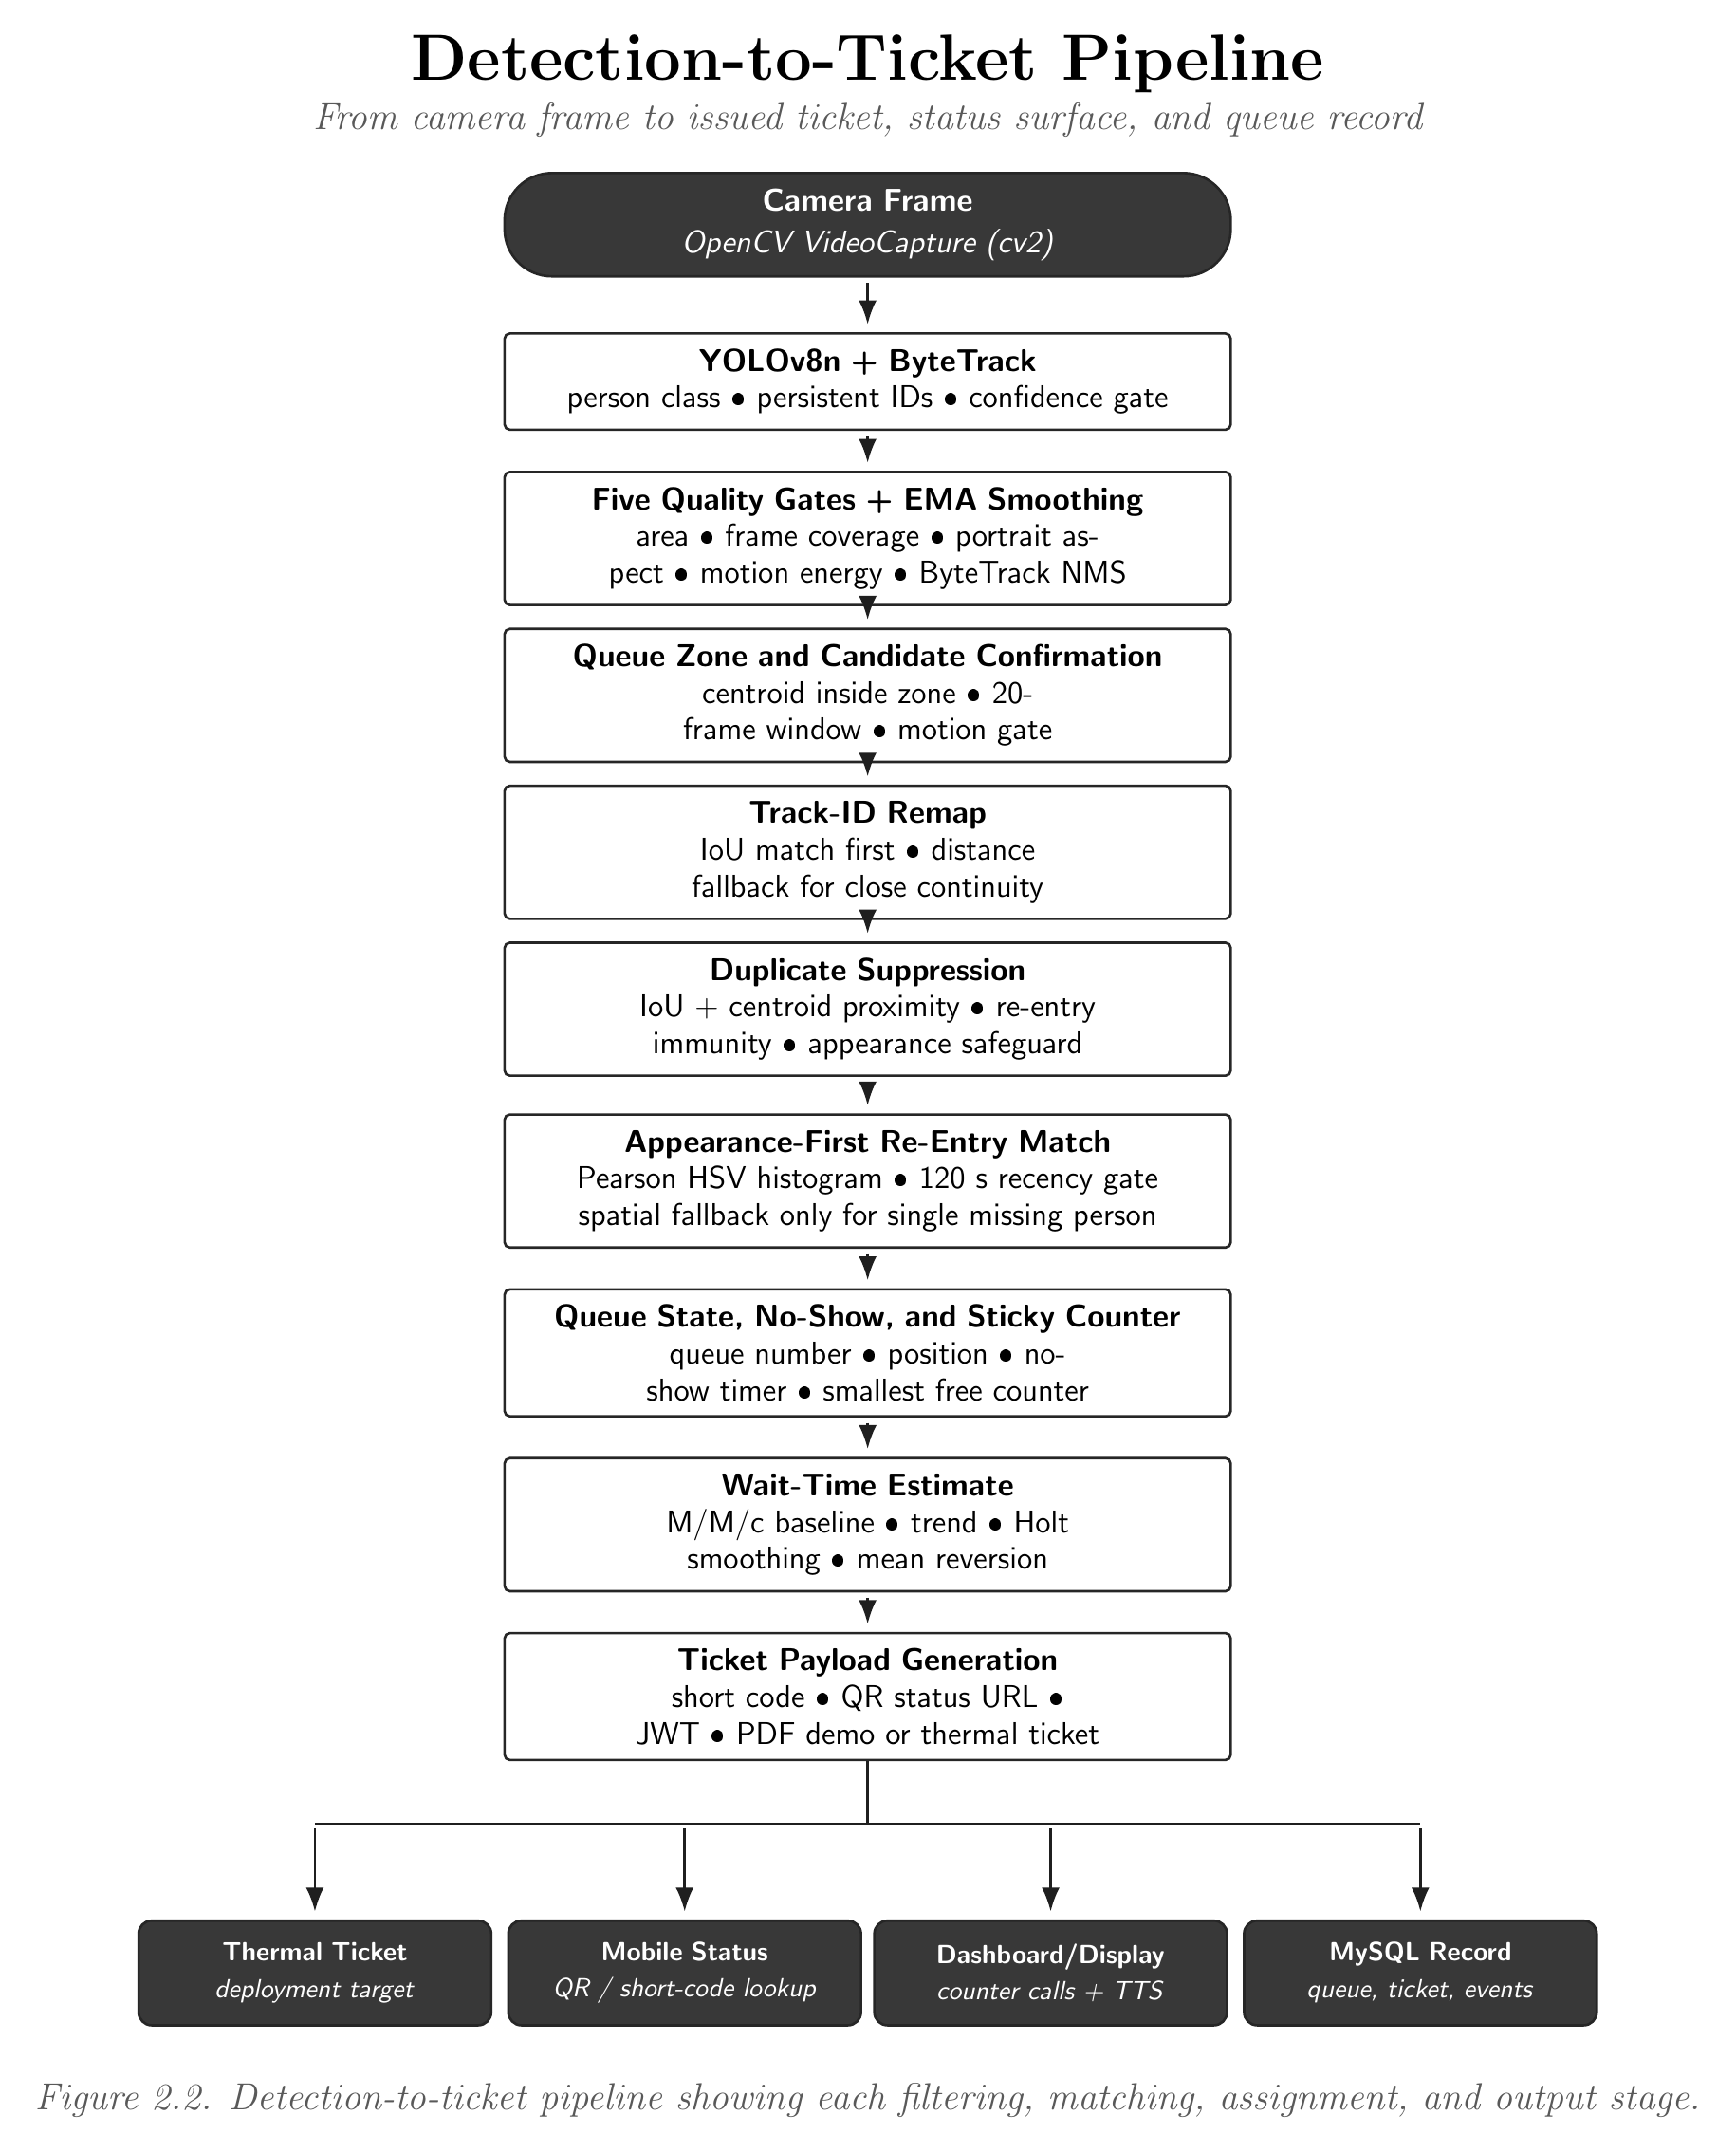
\begin{tikzpicture}[
  font=\sffamily,
  proc/.style={draw=black!85, line width=0.95pt, fill=white, align=center,
    rounded corners=2pt, text width=9.3cm, minimum height=1.25cm,
    inner sep=6pt, font=\sffamily\large},
  darkproc/.style={proc, fill=black!78, text=white, rounded corners=18pt},
  output/.style={darkproc, text width=4.3cm, minimum height=1.4cm, rounded corners=5pt, font=\sffamily\normalsize},
  arrow/.style={-{Latex[length=3.2mm]}, line width=0.95pt, black!88,
    shorten >=3pt, shorten <=2pt},
  branch/.style={line width=0.95pt, black!88}
]

\node[font=\bfseries\Huge] at (0,0) {Detection-to-Ticket Pipeline};
\node[font=\itshape\Large, text=black!65] at (0,-0.75)
  {From camera frame to issued ticket, status surface, and queue record};

\node[darkproc] (camera) at (0,-2.15)
  {\textbf{Camera Frame}\\[2pt]\textit{OpenCV VideoCapture (cv2)}};
\node[proc] (detect) at (0,-4.25)
  {\textbf{YOLOv8n + ByteTrack}\\person class \textbullet{} persistent IDs \textbullet{} confidence gate};
\node[proc] (quality) at (0,-6.35)
  {\textbf{Five Quality Gates + EMA Smoothing}\\area \textbullet{} frame coverage \textbullet{} portrait aspect \textbullet{} motion energy \textbullet{} ByteTrack NMS};
\node[proc] (zone) at (0,-8.45)
  {\textbf{Queue Zone and Candidate Confirmation}\\centroid inside zone \textbullet{} 20-frame window \textbullet{} motion gate};
\node[proc] (remap) at (0,-10.55)
  {\textbf{Track-ID Remap}\\IoU match first \textbullet{} distance fallback for close continuity};
\node[proc] (dedup) at (0,-12.65)
  {\textbf{Duplicate Suppression}\\IoU + centroid proximity \textbullet{} re-entry immunity \textbullet{} appearance safeguard};
\node[proc] (reid) at (0,-14.95)
  {\textbf{Appearance-First Re-Entry Match}\\Pearson HSV histogram \textbullet{} 120 s recency gate\\spatial fallback only for single missing person};
\node[proc] (queue) at (0,-17.25)
  {\textbf{Queue State, No-Show, and Sticky Counter}\\queue number \textbullet{} position \textbullet{} no-show timer \textbullet{} smallest free counter};
\node[proc] (predict) at (0,-19.55)
  {\textbf{Wait-Time Estimate}\\M/M/c baseline \textbullet{} trend \textbullet{} Holt smoothing \textbullet{} mean reversion};
\node[proc] (ticket) at (0,-21.85)
  {\textbf{Ticket Payload Generation}\\short code \textbullet{} QR status URL \textbullet{} JWT \textbullet{} PDF demo or thermal ticket};

\node[output] (thermal) at (-7.4,-25.55)
  {\textbf{Thermal Ticket}\\[2pt]\textit{deployment target}};
\node[output] (mobile) at (-2.45,-25.55)
  {\textbf{Mobile Status}\\[2pt]\textit{QR / short-code lookup}};
\node[output] (display) at (2.45,-25.55)
  {\textbf{Dashboard/Display}\\[2pt]\textit{counter calls + TTS}};
\node[output] (mysql) at (7.4,-25.55)
  {\textbf{MySQL Record}\\[2pt]\textit{queue, ticket, events}};

\foreach \a/\b in {camera/detect,detect/quality,quality/zone,zone/remap,remap/dedup,dedup/reid,reid/queue,queue/predict,predict/ticket}
  \draw[arrow] (\a) -- (\b);

\coordinate (split) at (0,-23.55);
\coordinate (thermalTop) at (-7.4,-23.55);
\coordinate (mobileTop) at (-2.45,-23.55);
\coordinate (displayTop) at (2.45,-23.55);
\coordinate (mysqlTop) at (7.4,-23.55);

\draw[branch] (ticket.south) -- (split);
\draw[branch] (thermalTop) -- (mysqlTop);
\draw[arrow] (thermalTop) -- (thermal.north);
\draw[arrow] (mobileTop) -- (mobile.north);
\draw[arrow] (displayTop) -- (display.north);
\draw[arrow] (mysqlTop) -- (mysql.north);

\node[font=\itshape\Large, text=black!65] at (0,-27.25)
  {Figure 2.2. Detection-to-ticket pipeline showing each filtering, matching, assignment, and output stage.};
\end{tikzpicture}
\end{document}
